\documentclass[border=10pt]{standalone}
\usepackage[svgnames]{xcolor}
\usepackage{amsmath}
\usepackage{pgfplots}
\pgfplotsset{compat=newest}
\usepackage[sfdefault]{FiraSans}
\usepackage{FiraMono}
\renewcommand*\familydefault{\sfdefault}
\begin{document}
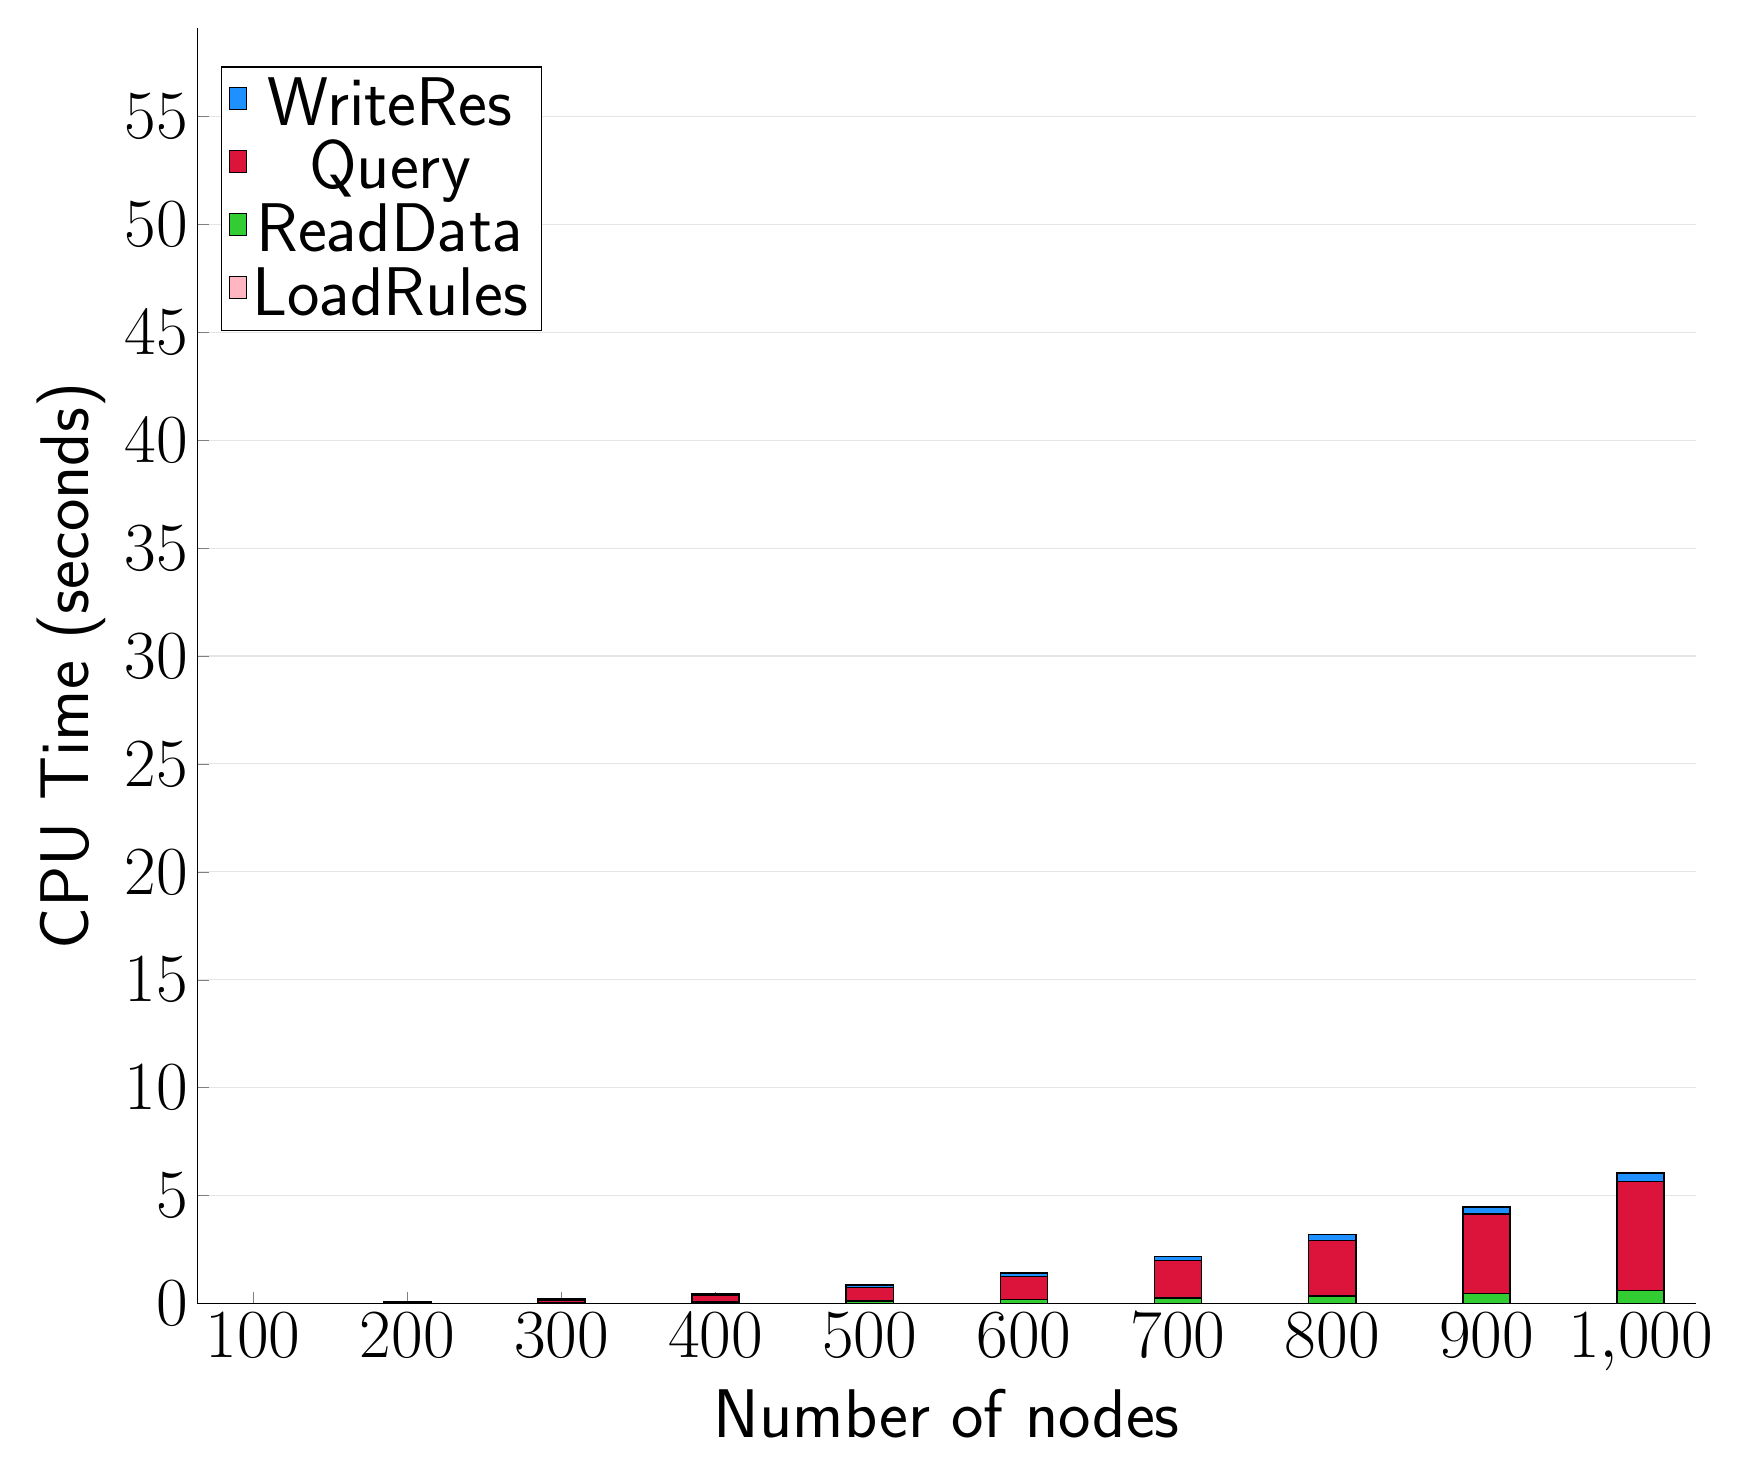
\begin{tikzpicture}
\begin{axis}[
   ybar stacked,
   width=1.7\textwidth,
   bar width=0.6cm,
   ymajorgrids, tick align=inside,
   major grid style={draw=gray!20},
   xtick=data,
   ymin=0, ymax=59.082040000000006,
   axis x line*=bottom,
   axis y line*=left,
   enlarge x limits=0.04,
   legend style={
       at={(0.23, 0.97)},
       anchor=north east,
       legend columns=1,
       font=\Huge,
   },
   ylabel={CPU Time (seconds)},
   xlabel={Number of nodes},
   label style={font=\Huge},
   tick label style={font=\Huge},
]
\addlegendimage{fill=DodgerBlue, draw=black, line width=0.2pt}
\addlegendentry{WriteRes}
\addlegendimage{fill=Crimson, draw=black, line width=0.2pt}
\addlegendentry{Query}
\addlegendimage{fill=LimeGreen, draw=black, line width=0.2pt}
\addlegendentry{ReadData}
\addlegendimage{fill=LightPink, draw=black, line width=0.2pt}
\addlegendentry{LoadRules}
\addplot +[fill=LightPink, draw=black, line width=0.55pt] coordinates {
(100, 0.0005546000000000003)
(200, 0.0005498)
(300, 0.0005532)
(400, 0.0005474)
(500, 0.0005608)
(600, 0.0005552000000000003)
(700, 0.0005568000000000003)
(800, 0.0005647999999999996)
(900, 0.0005519999999999998)
(1000, 0.0005498)
};
\addplot +[fill=LimeGreen, draw=black, line width=0.55pt] coordinates {
(100, 0.0040464)
(200, 0.0170404)
(300, 0.0404432)
(400, 0.0749182)
(500, 0.122499)
(600, 0.1830168)
(700, 0.26352580000000003)
(800, 0.3552006)
(900, 0.4698704)
(1000, 0.6045078)
};
\addplot +[fill=Crimson, draw=black, line width=0.55pt] coordinates {
(100, 0.00546)
(200, 0.041587799999999994)
(300, 0.1367956)
(400, 0.32369259999999994)
(500, 0.6321004)
(600, 1.0775756)
(700, 1.725069)
(800, 2.5780466)
(900, 3.6796127999999997)
(1000, 5.046770199999999)
};
\addplot +[fill=DodgerBlue, draw=black, line width=0.55pt] coordinates {
(100, 0.0038932000000000003)
(200, 0.015961400000000004)
(300, 0.0367108)
(400, 0.06519259999999999)
(500, 0.1022386)
(600, 0.1486462)
(700, 0.19131700000000001)
(800, 0.261694)
(900, 0.3297338000000001)
(1000, 0.3903354000000002)
};
\end{axis}
\end{tikzpicture}

\end{document}
